\begin{enumerate}
%1

\item \textbf{จงหาอนุพันธ์อันดับสองและสามของฟังก์ชันต่อไปนี้}
\begin{tasks}[after-skip = 100pt](4)
\task $f(x)=x^5$
\task $f(x) = \sqrt{x}$
\task $f(x) = \cos(3x)$
\task $f(x) = xe^x$
\end{tasks}

\item \textbf{อนุพันธ์เชิงเรขาคณิต}

สมการเส้นตรงที่สัมผัสเส้นโค้ง $y=f(x)$ ที่จุด $x=x_0$ คือ

\[ \blank[2] \]

จงหาสมการเส้นสัมผัสเส้นโค้ง ณ จุดที่กำหนดให้ต่อไปนี้ พร้อมวาดเส้นลงในกราฟด้วย

\begin{tasks}[after-skip = 120pt](3)
\task $y = x^2+4x$ ที่จุด $x = 1$

\begin{tikzpicture}[domain = -0.5:1.5]
\draw[<->] (-1,0) -- (2,0) node [right] {$x$};
\draw[<->] (0,-1) -- (0,2) node [above] {$y$};
\draw plot (\x, \x^2/5+4*\x/5);% node [right] {$y = x^2+4x$};
\end{tikzpicture}

\task $y = \ln x$ ที่จุด $x=1$

\begin{tikzpicture}[domain = 0.1:1.5]
\draw[<->] (-1,0) -- (2,0) node [right] {$x$};
\draw[<->] (0,-2) -- (0,1) node [above] {$y$};
\draw plot (\x, {ln(\x)});
\end{tikzpicture}

\task $y = \sin (3x)$ ที่จุด $x = \pi/6$

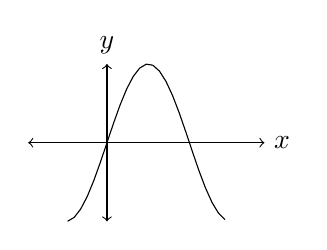
\begin{tikzpicture}[domain = -0.5:1.5]
\draw[<->] (-1,0) -- (2,0) node [right] {$x$};
\draw[<->] (0,-1) -- (0,1) node [above] {$y$};
\draw plot (\x, {sin(3*\x r)});
\end{tikzpicture}
\end{tasks}

\item \textbf{ฟังก์ชันเพิ่มและฟังก์ชันลด}

จงใช้อนุพันธ์เพื่อหาว่าฟังก์ชันต่อไปนี้เป็นฟังก์ชันเพิ่มในช่วงใด และเป็นฟังก์ชันลดในช่วงใด
\begin{tasks}[after-skip = 60pt](3)
\task $f(x)=x^4$
\task $f(x)=x-x^2$
\task $f(x)=e^x$
\end{tasks}

\newpage

\item \textbf{ความเว้า}

จงใช้อนุพันธ์อันดับสองเพื่อหาว่าฟังก์ชันต่อไปนี้เว้าบน (concave up) ในช่วงใด และเว้าล่าง (concave down) ในช่วงใด
\begin{tasks}[after-skip = 80pt](3)
\task $f(x)=x^3$
\task $f(x)=\ln x$
\task $f(x)=e^x$
\end{tasks}

\item \textbf{การหาและการทดสอบจุดวิกฤต}

$f(x)$ มีจุดวิกฤตที่จุด $(c, f(c))$ ก็ต่อเมื่อ \blank หรือ \blank 

\begin{itemize}
\item ถ้า $f\''(c) > 0$ แสดงว่าฟังก์ชันเว้า \rule{20pt}{0.5pt} จึงนับเป็นจุด \blank
\item ถ้า $f\''(c) < 0$ แสดงว่าฟังก์ชันเว้า \rule{20pt}{0.5pt} จึงนับเป็นจุด \blank
\item ถ้า $f\,''(c) = 0$ ให้สรุปว่า \blank
\end{itemize}

จงหาจุดวิกฤตทั้งหมดของฟังก์ชันต่อไปนี้ พร้อมทดสอบว่าเป็นจุดประเภทใด
\begin{tasks}[after-skip = 100pt](3)
\task $f(x)=x^2-10x$
\task $f(x)=x^3-3x^2$
\task $f(x)=x^4-1$
\end{tasks}

\item \textbf{โจทย์ปัญหาค่าสุดขีด}

\begin{tasks}[after-item-skip = 100pt, after-skip = 100pt](1)
\task มีที่ดินติดแม่น้ำอยู่ ให้ล้อมรั้วไม้ยาว 60 เมตรให้เป็นรูปสี่เหลี่ยมผืนผ้าที่มีพื้นที่มากที่สุด โดยล้อมเพียง 3 ด้าน ให้ด้านที่ 4 เป็นริมแม่น้ำ
\task สร้างกล่องสี่เหลี่ยมให้ฝาและก้นเป็นรูปสี่เหลี่ยมจัตุรัส ให้ได้ปริมาตร 1,000 ลูกบาศก์เซนติเมตรและราคาถูกที่สุด โดยฝาและก้นทำจากพลาสติกที่มีค่าใช้จ่ายตารางเซนติเมตรละ 20 บาท และด้านข้างเป็นกระดาษที่มีค่าใช้จ่ายตารางเซนติเมตรละ 10 บาท
\end{tasks}
\end{enumerate}

\end{document}